\chapter{Copula Multivariate Model}
\label{chap:5}

The previous chapters covered various approaches to modeling univariate asset returns. These univariate methods can also be applied directly to portfolio returns. However, while modeling aggregate portfolio returns is suitable for passive risk measurement, it offers limited insight for active risk management. To conduct sensitivity analyses and evaluate diversification benefits, it is necessary to model the dependence structure between individual asset returns. This chapter discusses the copula approach for constructing multivariate risk models.

Alternative approaches to modeling a set of assets (multivariate risk) include those based on the Dynamic Conditional Correlation (DCC) model, which captures the linear dependence between standardized asset returns. A key strength of the DCC approach is its ability to reflect the dynamic correlation patterns introduced in \hyperref[chap:1]{Chapter 1} and illustrated in Figure~\ref{5.1}. Additionally, the DCC model can be combined with multivariate distributions designed to capture asymmetry and heavy tails—features previously discussed in a univariate context but now extended to multiple dimensions. Readers interested in exploring this approach in detail are encouraged to consult \citeA{Christoffersen2012}, which provides a comprehensive overview of the DCC model and compatible multivariate densities.

\begin{figure}[H]
    \centering
    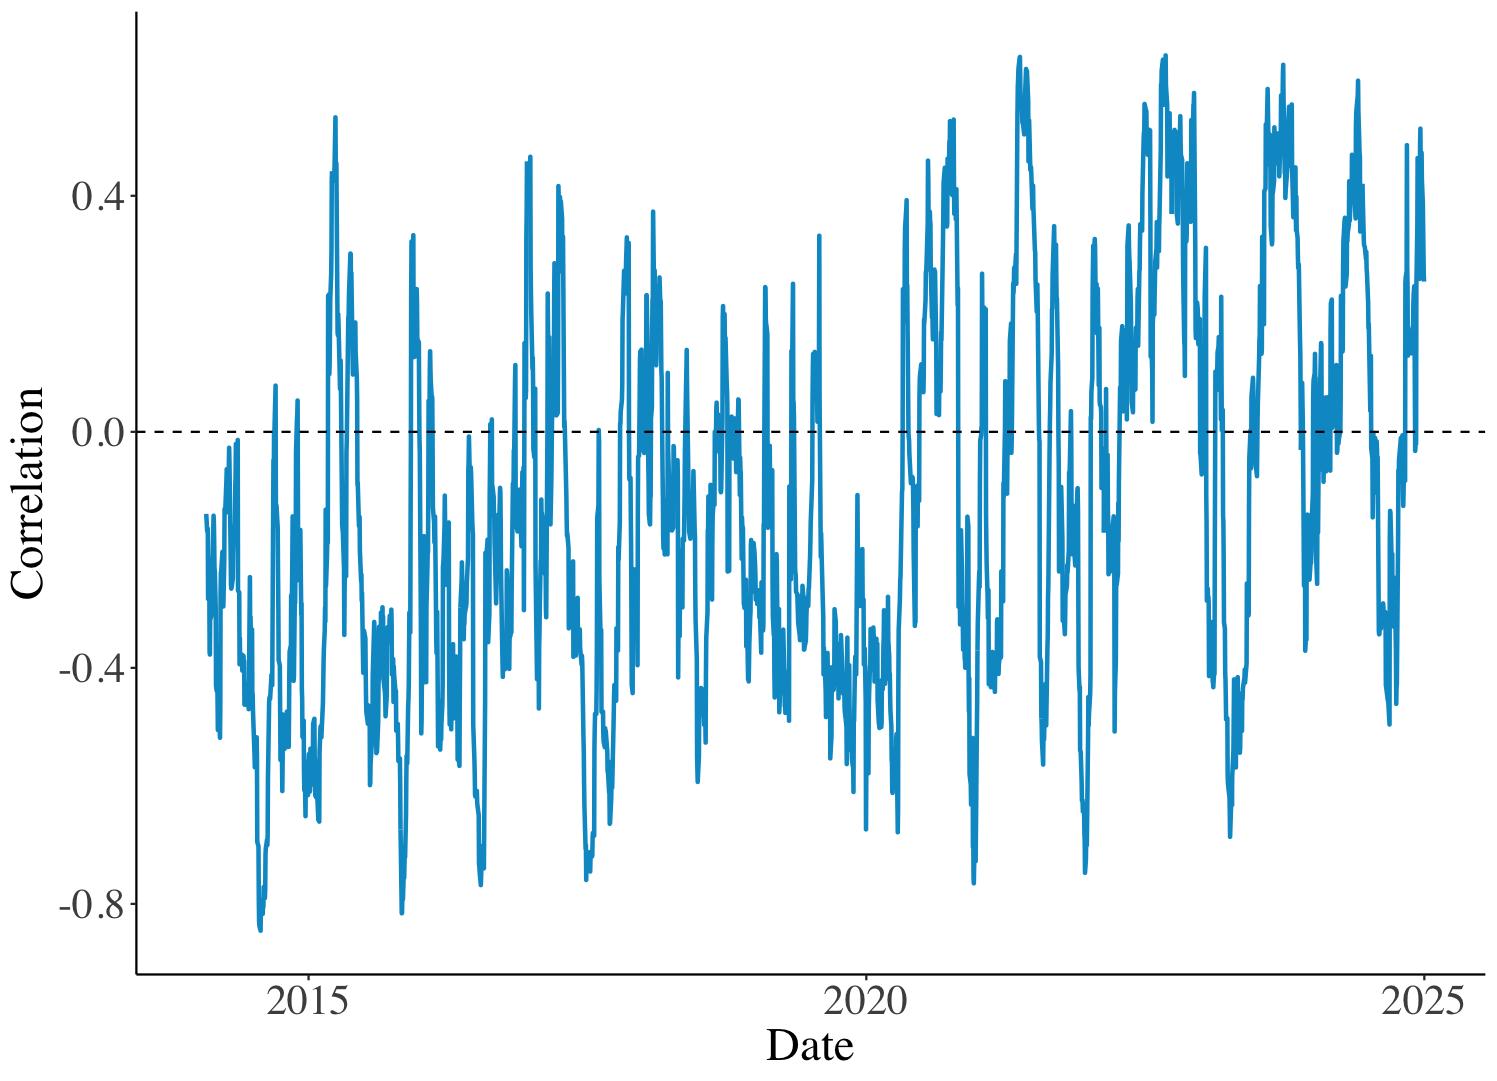
\includegraphics[scale=0.18]{../../plots/5.1.png} % Replace 
   \caption{25-day rolling correlation between the standardized returns of the S\&P 500 and the 10-year Treasury note index (training period).}
    \label{5.1}
\end{figure}

The DCC model approach has two key limitations. First, it focuses exclusively on capturing linear dependencies, thus overlooking more complex nonlinear relationships—particularly in the tails of asset distributions, which are critical for effective risk management. Second, it constrains the univariate models by tying their parameters directly to those estimated within the multivariate framework, potentially limiting their ability to accurately represent individual asset behavior.

The copula modeling approach addresses these issues. It can capture both linear and nonlinear dependencies effectively and allows for separate, flexible univariate models for each asset. These individual univariate models serve as inputs to the copula—analogous to ingredients being blended—resulting in a multivariate model that preserves each asset’s distinctive univariate properties.

Although copula models can be specified dynamically, this chapter employs a static copula for the standardized returns, following \citeA{jondeau2006copulagarch}. In this static specification, the copula parameters are time-invariant (e.g., in a $t$-copula the correlation parameter $\rho^*$ and the degrees of freedom $d$ do not vary with $t$); any dynamics arise solely from the marginal models. Consequently, the specification does not capture time variation in cross-asset dependence (e.g., dynamic correlations). Dynamic copula models have been extensively developed by \citeA{patton2006modelling}, \citeA{patton2011factor}, and \citeA{christoffersen2011joint}. In particular, \citeA{christoffersen2011joint} embed Dynamic Conditional Correlation dynamics within the copula, yielding time-varying dependence.

From a risk management perspective, the tail dependence between assets warrants particular attention. A portfolio containing assets with strongly correlated left-tail returns could suffer significant losses during sharp market downturns. To visualize such tail dependencies, threshold correlations play a key role. The threshold correlation between two standardized returns $z_{1,t}$ and $z_{2,t}$ at level $p$ is defined as
\begin{equation}
\rho(r_{1,t}, r_{2,t}; p) =
\begin{cases}
\text{Corr}\left(z_{1,t}, z_{2,t} \mid z_{1,t} \leq z_1(p) \text{ and } z_{2,t} \leq z_2(p)\right), & \text{if } p \leq 0.5 \\[0.5em]
\text{Corr}\left(z_{1,t}, r_{2,t} \mid z_{1,t} > z_1(p) \text{ and } z_{2,t} > z_2(p)\right), & \text{if } p > 0.5
\end{cases}
\label{eq:5.1}
\end{equation}


where $z_{i}(p)$ represents the $p$-th percentile of the standardized returns of asset $i$.

In other words, the threshold correlation measures the correlation between two assets conditioned on both returns being simultaneously below their respective $p$-th percentiles (for $p<0.5$) or above these percentiles (for $p>0.5$). Calculating threshold correlations across a range of $p$-values and plotting these correlations yields the threshold correlation plot. As noted by \citeA{Christoffersen2012}, threshold correlations reveal how asset returns behave jointly during extreme events—large negative or positive returns—thus providing insights into the shape of the tails of their joint distribution.

Figure~\ref{5.2} displays the threshold correlation plot between the S\&P 500 returns and the 10-year Treasury bond returns standardized by their respective GARCH(1,1) volatilities. For values of $p$ close to 0 or 1, the number of observations becomes limited, which prevents reliable correlation estimation; thus, only correlations computed with at least 25 observations are presented. Although the extreme correlations exhibit considerable variability and should be interpreted cautiously, an important pattern emerges clearly: correlations increase as returns move deeper into the tails. This indicates a heavy-tailed bivariate distribution between stock and bond returns. Additionally, note that there is asymmetry in the tail dependence, the right tail exhibits a higher correlation.

\begin{figure}[H]
    \centering
    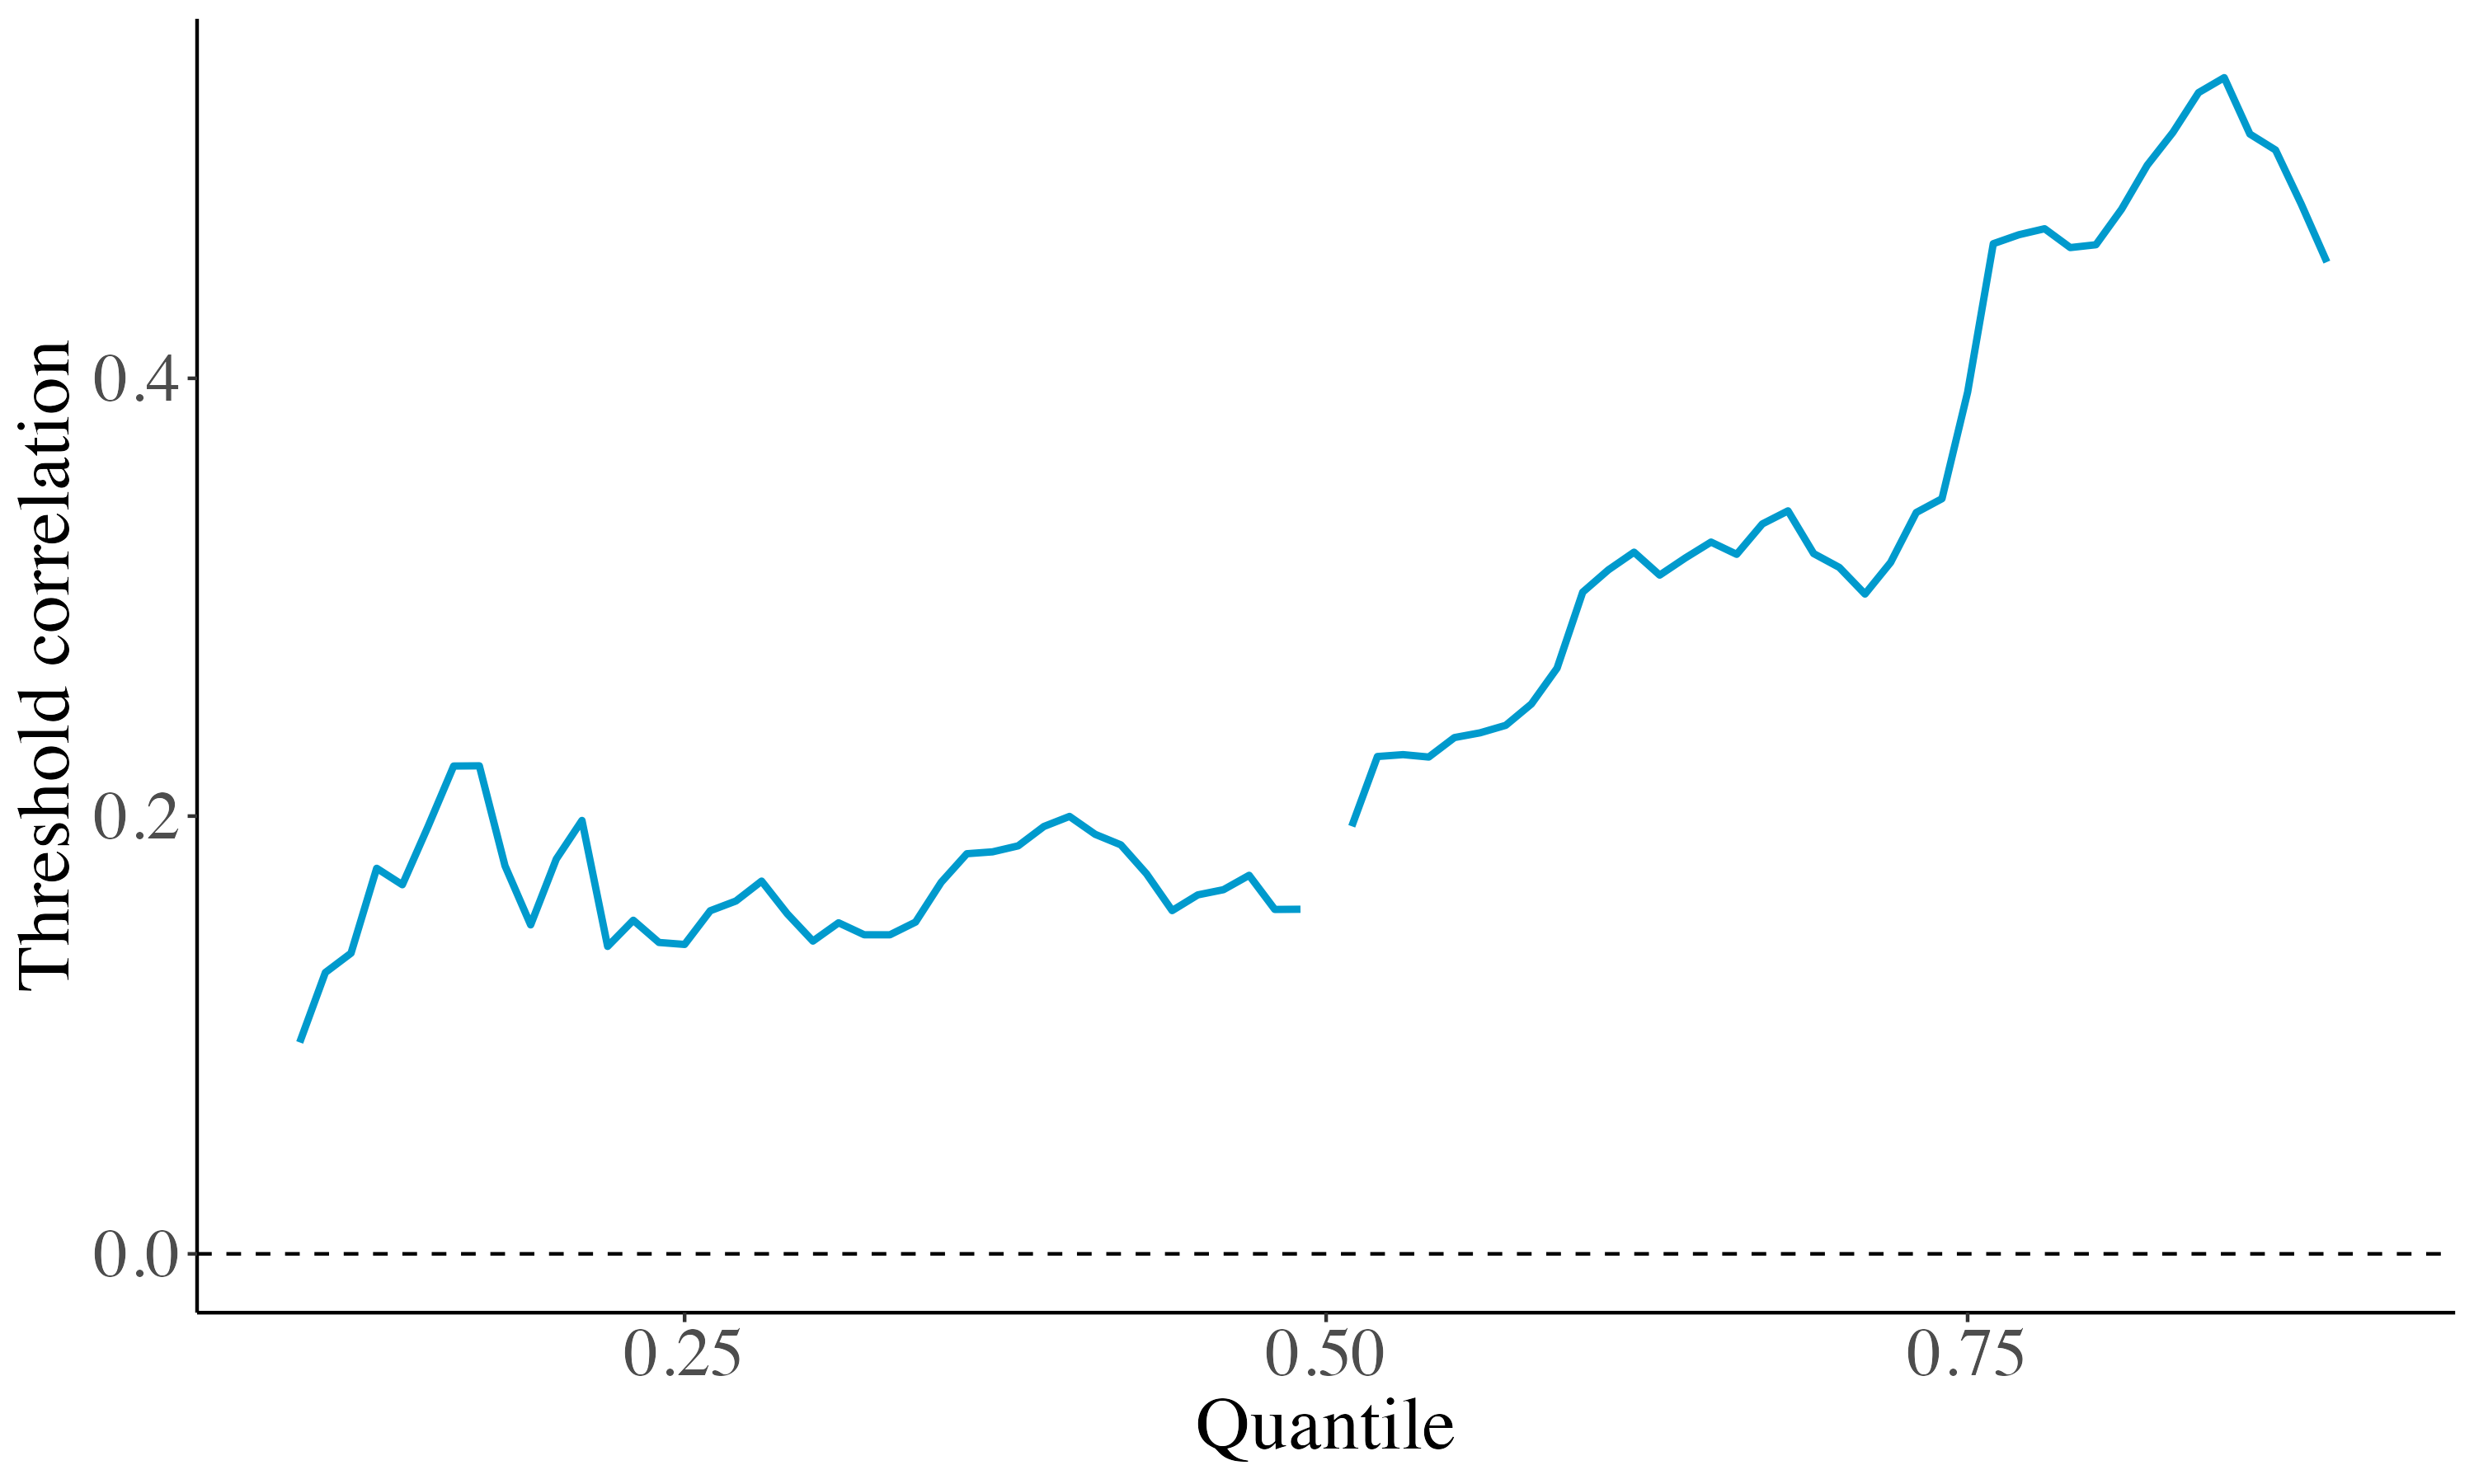
\includegraphics[scale=0.43]{../../plots/5.2.png} % Replace 
   \caption{Threshold correlation of GARCH(1,1) standardized returns (training period).}
    \label{5.2}
\end{figure}

Such tail dependence exemplifies the nonlinear relationships that the copula modeling approach aims to capture and replicate. The results in Figure~\ref{5.2} underscore the importance of modeling nonlinear left-tail dependencies between stocks and bonds. An influential application of threshold correlations is provided by \citeA{okimoto2008asymmetric}, who investigates asymmetric dependence structures among international equity markets.

Following the exposition by \citeA{Christoffersen2012}, the theoretical foundation for copula models is provided by Sklar’s theorem. Consider $n$ assets and their respective standardized returns $z_i$, each with potentially distinct marginal probability density functions (PDFs) $f_i(z_i)$ and cumulative distribution functions (CDFs) $u_i=F_i(z_i)$ for $i = 1, 2, \ldots, n$. Sklar’s theorem states that for a very general class of multivariate cumulative distribution functions $ F(z_1, \ldots, z_n)$ with marginals $ F_1(z_1), \ldots, F_n(z_n)$, there exists a unique copula function $G(\cdot)$ that links these marginals to form the joint distribution:
\[
F(z_1, \dots, z_n) = G(F_1(z_1), \dots, F_n(z_n)) = G(u_1, \dots, u_n).
\]
The function $G(u_1, \dots, u_n)$ is referred to as the copula CDF. In line with Sklar’s theorem, the corresponding multivariate probability density function (PDF) can be expressed as:
\[
\begin{aligned}
f(z_1, \dots, z_n) &= \frac{\partial^n G(F_1(z_1), \dots, F_n(z_n))}{\partial z_1 \cdots \partial z_n} \\
&= \frac{\partial^n G(u_1, \dots, u_n)}{\partial u_1 \cdots \partial u_n} \times \prod_{i=1}^n f_i(z_i) \\
&= g(u_1, \dots, u_n) \times \prod_{i=1}^n f_i(z_i),
\end{aligned}
\]
where the copula PDF $g(u_1, \dots, u_n)$ is defined by:
\[
g(u_1, \dots, u_n) \equiv \frac{\partial^n G(u_1, \dots, u_n)}{\partial u_1 \cdots \partial u_n}.
\]
Taking logarithms simplifies the representation as follows:
\[
\ln f(z_1, \dots, z_n) = \ln g(u_1, \dots, u_n) + \sum_{i=1}^n \ln f_i(z_i).
\]

This decomposition demonstrates that constructing a complex multivariate density can be performed in two steps. First, individual marginal distributions $f_1(z_1), \ldots, f_n(z_n)$ are estimated independently using methods outlined in previous chapters. Second, the copula density function g$(u_1, \ldots, u_n)$ is chosen and estimated using the marginal probability values $u_i$ as input data.
\newpage
An important practical advantage of this method is that it simplifies parameter estimation: the parameters of the marginal distributions are estimated independently first, reducing the copula estimation to a separate, simpler second step. This property makes high-dimensional modeling feasible and efficient.

While Sklar’s theorem is quite general, holding true for a broad class of multivariate distributions, it does not specify a functional form for $G(u_1, \ldots, u_n)$. Therefore, an appropriate copula model must be selected based on the application and underlying data.

The $t$-copula, widely used in the literature (see, for instance, \citeA{christoffersen2011joint}),can be extended naturally to $n$ assets and, as will be demonstrated subsequently, is capable of reproducing reasonably the threshold correlations shown in Figure~\ref{5.2}. For these reasons, the $t$-copula is selected for our analysis. However, it is important to highlight that \citeA{okimoto2008asymmetric} finds evidence of significant asymmetric dependence structures in financial data, which symmetric copulas—such as Gaussian and $t$-copulas—may fail to fully capture.

The cumulative distribution function of the bivariate $t$-copula is defined as:
\begin{equation}
G(u_1, u_2; \rho^*, d) = t_{(d, \rho^*)} \left( t^{-1}(u_1; d), \, t^{-1}(u_2; d) \right)
\label{eq:5.2}
\end{equation}
where $t_{(d,\rho^*)}(\cdot)$ denotes the (non-standardized) symmetric multivariate $t$-distribution, $t^{-1}(u; d)$ is the inverse CDF of the (non-standardized) symmetric univariate $t$-distribution, and $\rho^*$ is the correlation parameter between $t^{-1}(u_1; d)$ and $t^{-1}(u_2; d)$, commonly known as the copula correlation.

The corresponding probability density function or the bivariate $t$-copula is:
\begin{equation}
\begin{aligned}
g(u_1, u_2; \rho^*, d) &= \frac{
    t_{(d, \rho^*)}(t^{-1}(u_1; d), \, t^{-1}(u_2; d))
}{
    f_{t(d)}(t^{-1}(u_1; d); d) \, f_{t(d)}(t^{-1}(u_2; d); d)
} \\
&= \frac{
    \Gamma\left(\frac{d+2}{2}\right)
}{
    \sqrt{1 - (\rho^*)^2} \, \Gamma\left(\frac{d}{2}\right)
}
\left(
\frac{\Gamma\left(\frac{d}{2}\right)}{\Gamma\left(\frac{d+1}{2}\right)}
\right)^2 \\
&\quad \times
\frac{\left(
1 + \frac{(t^{-1}(u_1; d))^2 + (t^{-1}(u_2; d))^2 - 2\rho^* \, t^{-1}(u_1; d)t^{-1}(u_2; d)}
{d(1 - (\rho^*)^2)}
\right)^{-\frac{d+2}{2}}}
{
\left(
1 + \frac{(t^{-1}(u_1; d))^2}{d}
\right)^{\frac{d+1}{2}}
\left(
1 + \frac{(t^{-1}(u_2; d))^2}{d}
\right)^{\frac{d+1}{2}}},
\end{aligned}
\label{eq:5.3}
\end{equation}
where $f_{t(d)}(\cdot; d)$ denotes the PDF of the symmetric univariate $t$-distribution with $d$ degrees of freedom.

The $t$-copula will be fitted to the standardized returns of two assets: the S\&P 500 and the 10-year Treasury note index (Bloomberg ticker: SPBDU1BT Index). The estimation period spans January 2014 to December 2024, matching the training period used previously for the S\&P 500 returns. Initially, univariate models are fitted separately to each asset following the framework outlined in earlier chapters, namely, a volatility model combined with a density model for the standardized asset returns. Because the copula approach requires complete density forecasts as inputs, only the asymmetric $t$-distribution—among the models discussed in \hyperref[chap:3]{Chapter 3}—is considered here. Table~\ref{tab:5.1} presents the estimated parameters of the GARCH-Asyt and GJR-Asyt models applied to the Treasury note index, following the specification given in Equations~\eqref{eq:3.2}, \eqref{eq:3.3}, and \eqref{eq:3.4}.

\begin{table}[H]
\footnotesize
\centering
\begin{tabular}{lcccccc}
\toprule
\textbf{Model} & $\omega$ & $\alpha$ & $\beta$ & $\theta$ & $d_1$ & $d_2$ \\
\midrule
GARCH-Asyt &  $3.46 \mathrm{e}{-7}$ & 0.007 & 0.92 & - & 11.01 & $7.5 \mathrm{e}{-3}$ \\
GJR-Asyt & $3.97\mathrm{e}{-7}$ & 0.007 &  0.91 & 0.0344 &  10.97 &  0.0021 \\
\bottomrule
\end{tabular}
\caption{Bond index estimated parameters.}
\label{tab:5.1}
\end{table}
For each asset, two sets of standardized returns are obtained based on the GARCH(1,1) and GJR(1,1) specifications. This yields four potential copula model combinations. To simplify the analysis, only two cases are considered: i) both assets follow the GARCH-Asyt model, and ii) both follow the GJR-Asyt model. Table~\ref{tab:5.2} reports the fitted copula parameters of the GARCH-GARCH and GJR-GJR models. 
\begin{table}[H]
\footnotesize
\centering
\begin{tabular}{lcc}
\toprule
\textbf{Copula model} & $\rho^*$ & $d$ \\
\midrule
GARCH-GARCH &  $-0.2121$ & 4.9671  \\
GJR-GJR & $-0.2088$ & 4.8304  \\
\bottomrule
\end{tabular}
\caption{Copula models estimated parameters.}
\label{tab:5.2}
\end{table}
Using the estimated copula model, it is possible to simulate data and examine whether the model-implied threshold correlations match the empirical pattern observed in Figure \ref{5.2}. Figures~\ref{5.3} and \ref{5.4} display the simulated threshold correlations obtained from the GARCH-GARCH and GJR-GJR copula models, respectively, alongside the empirical threshold correlations derived from the standardized returns. The $t$-copula successfully reasonably replicates the increasing correlation observed in the tails. However, it is worth mentioning that the standardized returns exhibit slightly higher correlation in the right tail, a subtle feature the symmetric $t$-copula cannot fully replicate.
\begin{figure}[H]
    \centering
    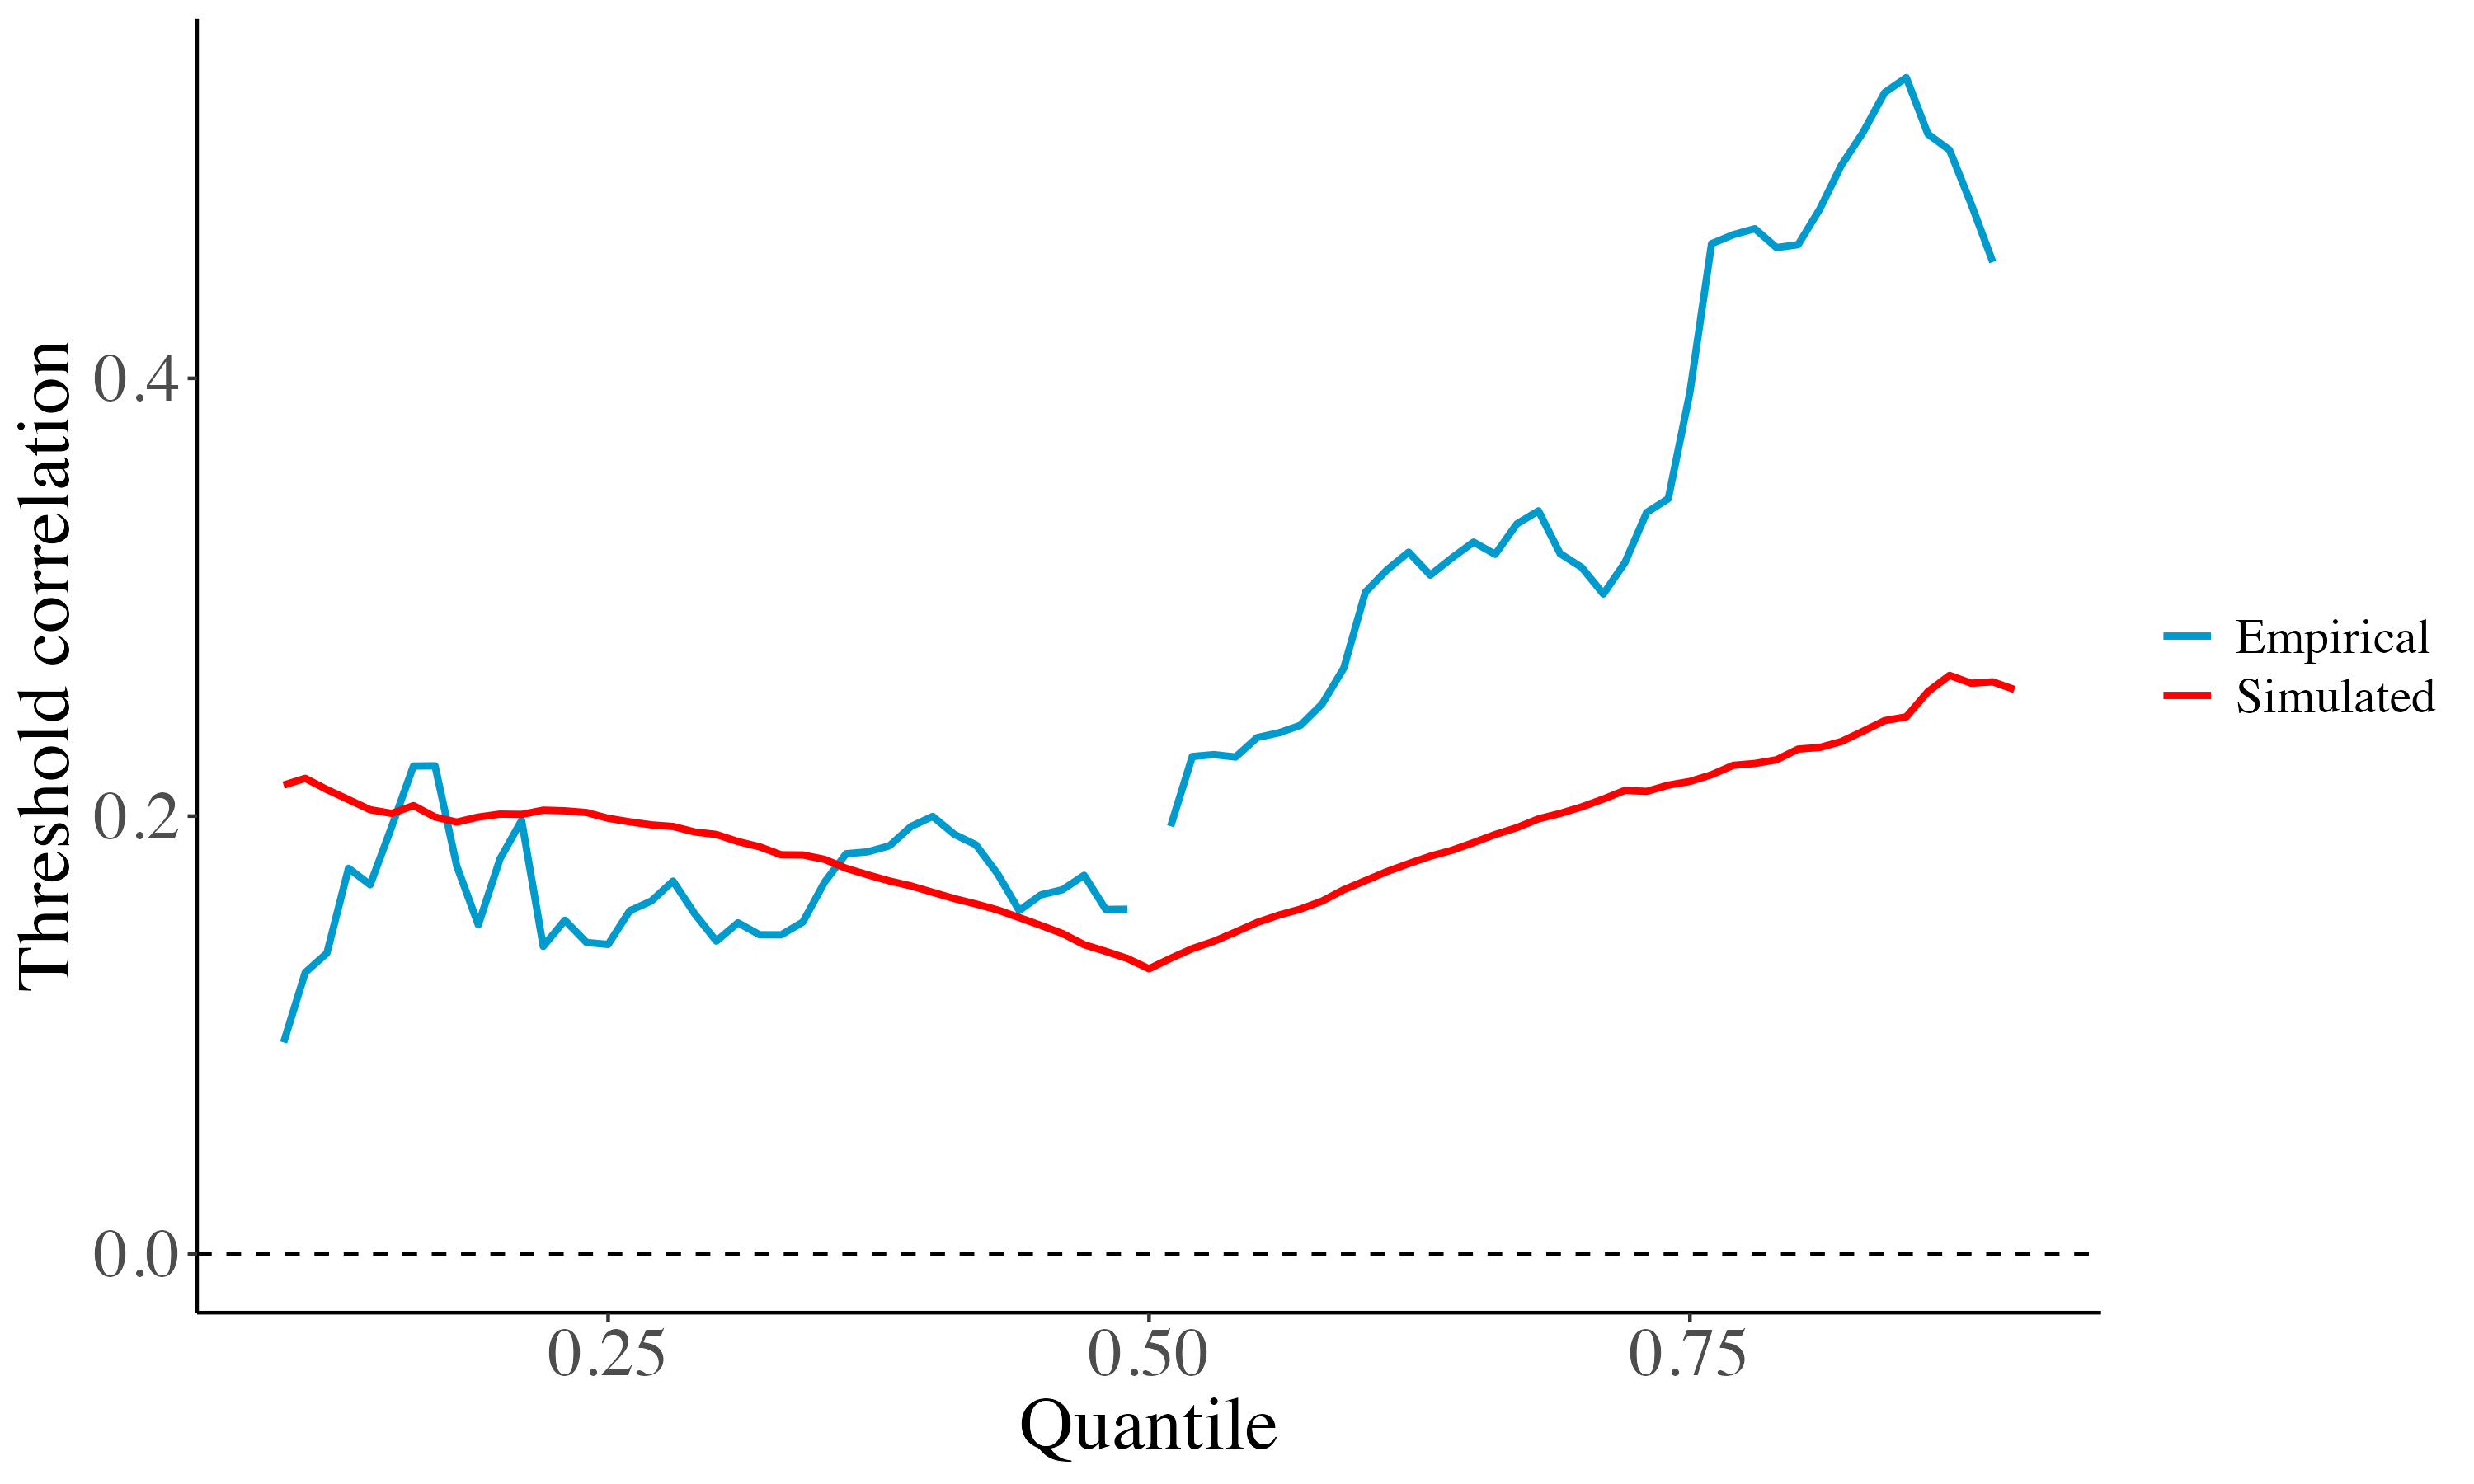
\includegraphics[scale=0.43]{../../plots/5.3.png} % Replace 
   \caption{Empirical and simulated threshold correlations of GARCH-GARCH copula.}
    \label{5.3}
\end{figure}

\begin{figure}[H]
    \centering
    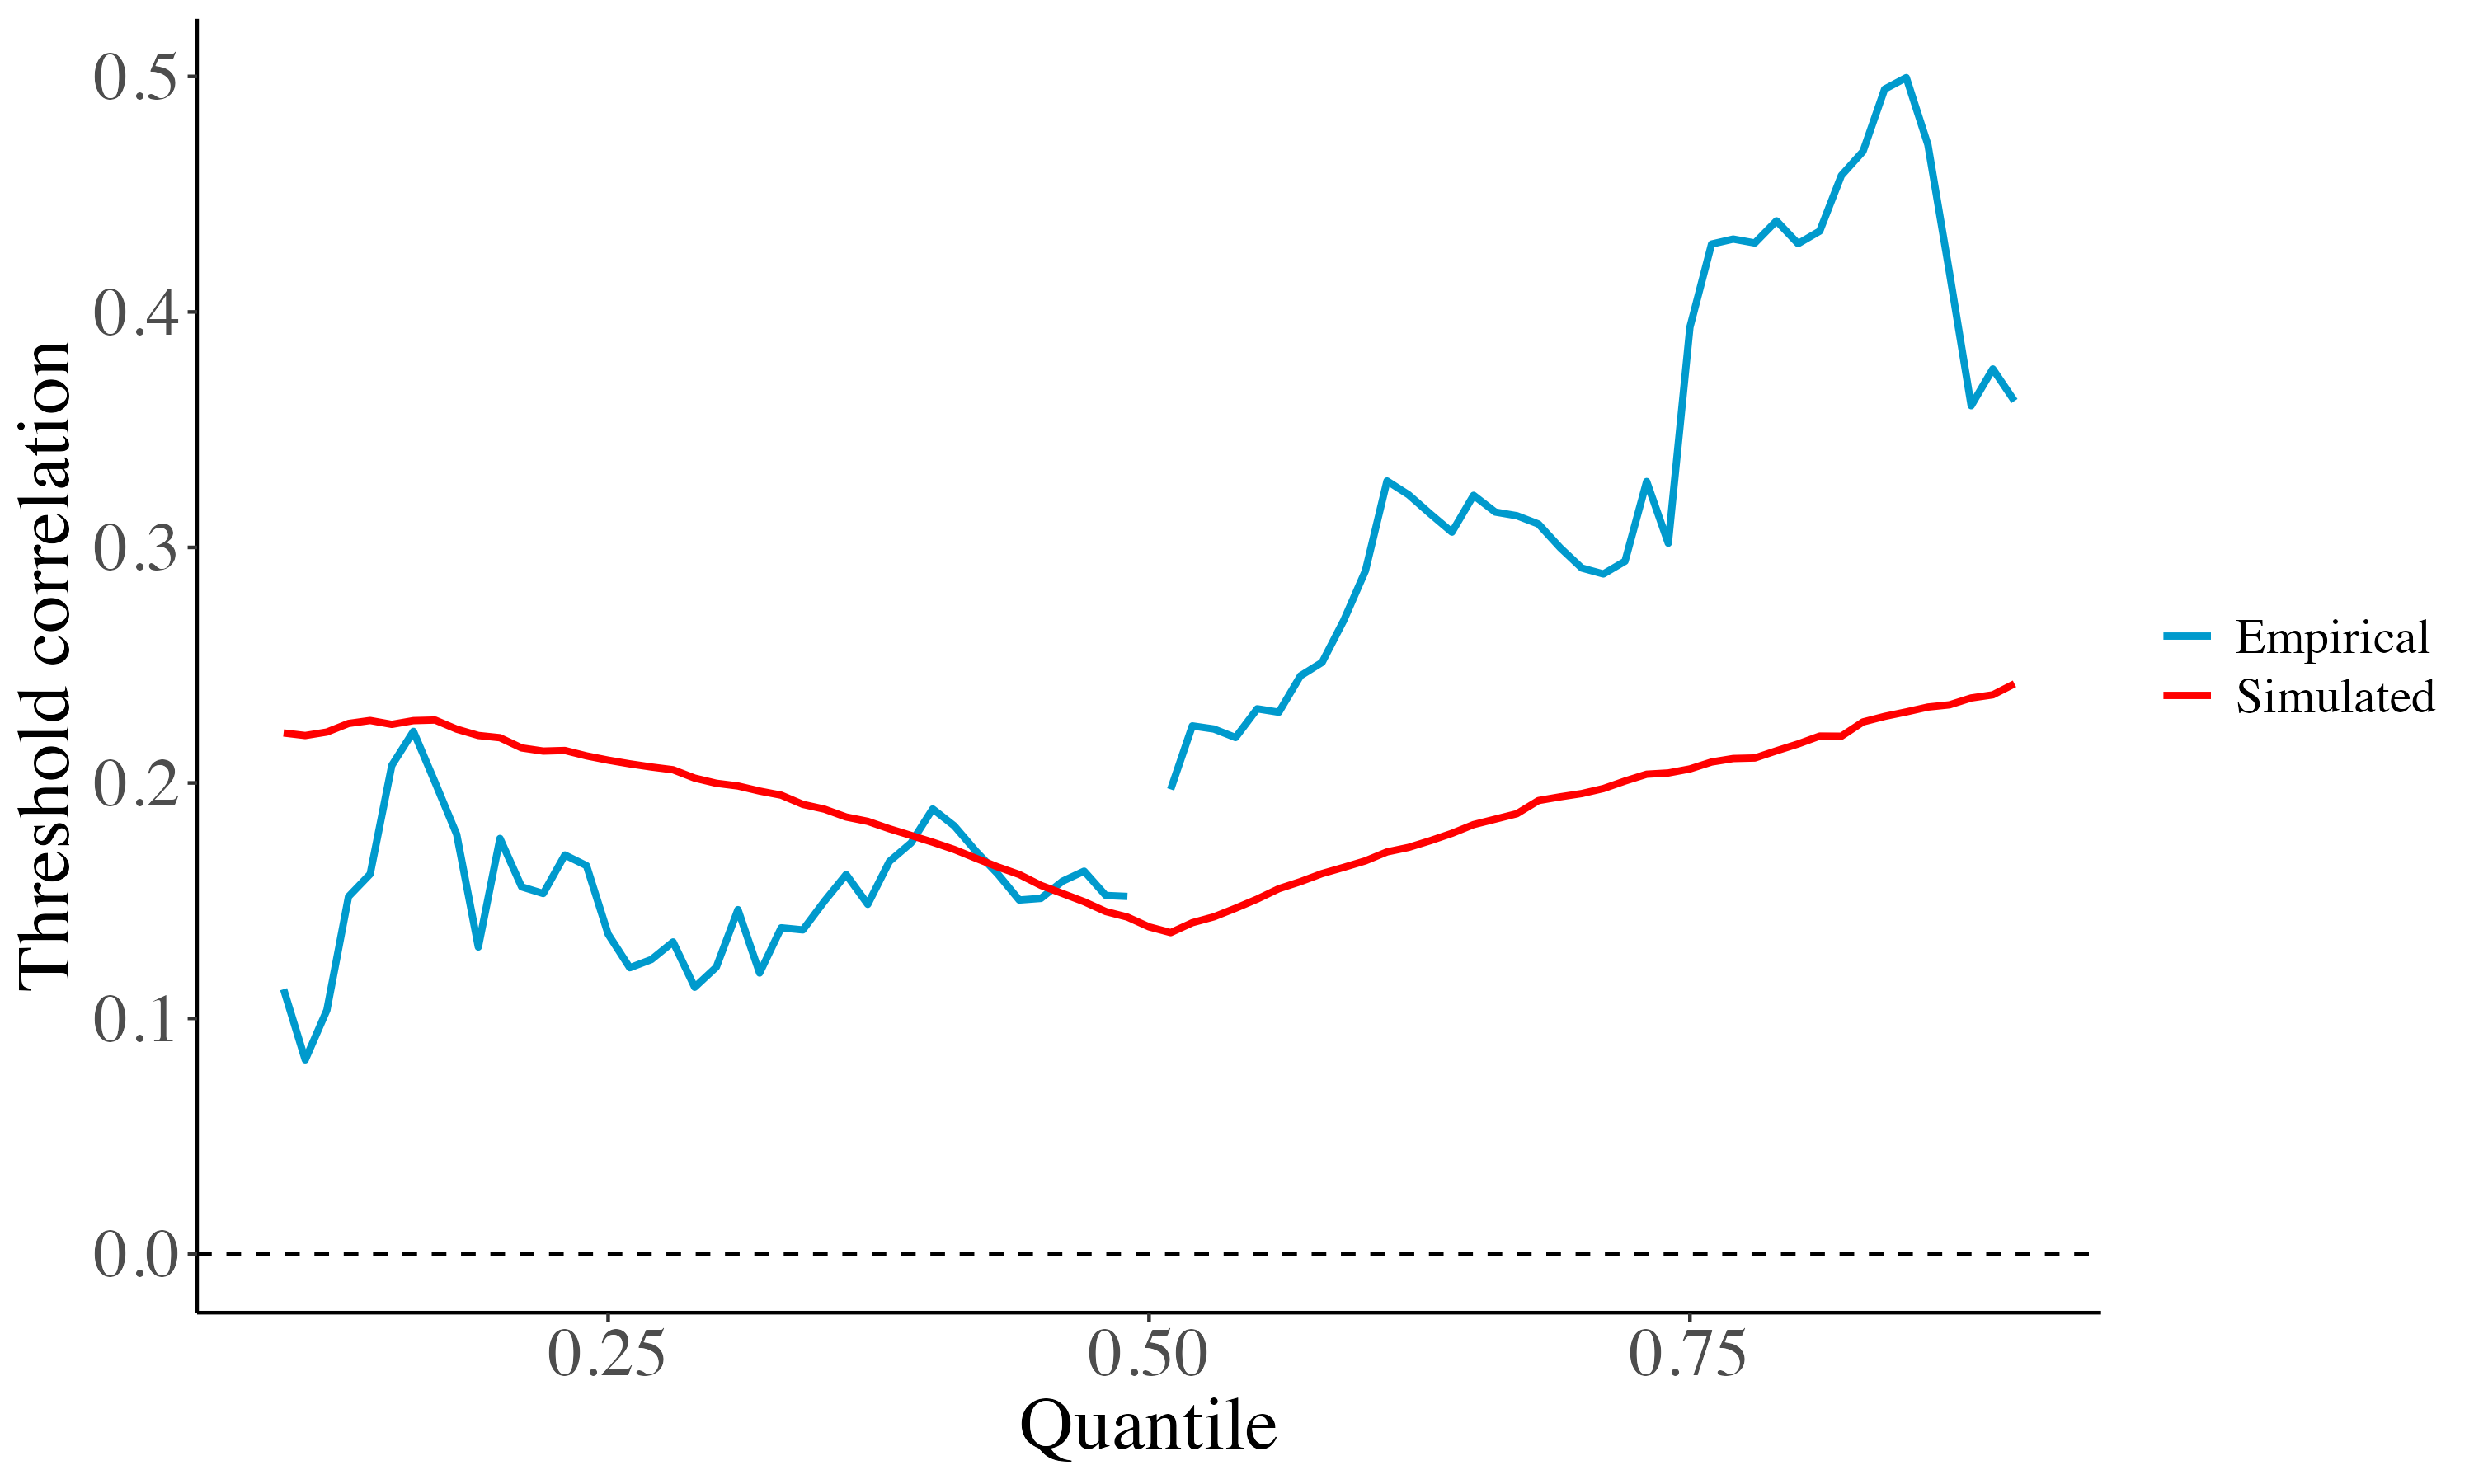
\includegraphics[scale=0.43]{../../plots/5.4.png} % Replace 
   \caption{Empirical and simulated threshold correlations of GJR-GJR copula.}
    \label{5.4}
\end{figure}

As shown by \citeA{christoffersen2011joint}, dynamic and static asymmetric copulas can match the empirical behavior of threshold correlations and thus offer a powerful alternative to the approach used in this chapter.

The subsequent step is to evaluate the forecasting performance of the copula models. Consider an equally-weighted portfolio composed of the S\&P 500 and the bond index. The validity of the multivariate copula models and their effectiveness from a risk management perspective will be assessed using this hypothetical portfolio.

Due to the complexity of the multivariate setup, closed-form expressions for the next day’s portfolio density forecast, VaR, and ES are no longer feasible. Consequently, a Monte Carlo approach is used. The algorithm is as follows:
\begin{enumerate}
\item[i.] At the end of trading day $t$, observed returns $R_{1,t}$ and $R_{2,t}$ are used to forecast the next day’s conditional volatilities $\sigma_{1,t+1}$ and $\sigma_{2,t+1}$, applying either the fitted GARCH or GJR volatility specification.
\item[ii.] Draw $M$ simulated probability pairs $(\check{u}_{1,t+1}, \check{u}_{2,t+1})$ from the fitted copula model.
\item[iii.] Transform these simulated copula probabilities into standardized shocks using the inverse of the fitted marginal distributions: $\check{z}_{i,t+1} = F_i^{-1}(\check{u}_{i,t+1}), \quad i=1,2$.
\item[iv.] Generate asset returns by scaling these shocks with the forecasted volatilities: $\check{R}_{i,t+1} = \sigma_{i,t+1} \check{z}_{i,t+1}, \quad i=1,2$.
\end{enumerate}
\newpage
After simulating $M$ scenarios of next-day returns for each asset, the corresponding portfolio returns are easily computed based on the given portfolio weights. Risk measures, including portfolio VaR and ES, can then be derived from the simulated distribution of portfolio returns. Specifically, the portfolio VaR at the 2.5\% level is estimated as the empirical 2.5th percentile of the simulated portfolio returns. Consequently, at the end of each trading day, the VaR forecast and associated simulated density of the portfolio returns can be obtained.

To further illustrate the simulation procedure, consider the case of a single asset. Figure~\ref{5.5} depicts the structure of the Monte Carlo algorithm used to simulate hypothetical next-day returns. Starting from the observed return at time $t$, the conditional variance forecast $\sigma^2_{t+1}$ is obtained using a GARCH or GJR specification. Next, draws are generated from the fitted copula to obtain simulated copula probabilities $\check{u}_{i,t+1}$, which are then transformed into shocks $\check{z}_{i,t+1}$ using the inverse of the marginal CDF. Finally, the shocks are scaled by the forecasted volatility to produce simulated returns $\check{R}_{i,t+1}$.

\begin{figure}[H]
\centering
\begin{tikzpicture}[
  every node/.style={align=center},
  arrow/.style={->, >=latex},
  base/.style={minimum height=0.8cm},
  label/.style={font=\color{miAzul}},
]

% Simulation path nodes (right side)
\node[base] (z11) at (4.5,1.4) {$\check{u}_{1,t+1} \rightarrow \check{z}_{1,t+1} \rightarrow \check{R}_{1,t+1}$};
\node[base] (z21) at (4.5,0.5) {$\check{u}_{2,t+1} \rightarrow \check{z}_{2,t+1} \rightarrow \check{R}_{2,t+1}$};
\node[base] (dots1) at (4.5,-0.1) {$\vdots$};
\node[base] (zmc1) at (4.5,-0.7) {$\check{u}_{M,t+1} \rightarrow \check{z}_{M,t+1} \rightarrow \check{R}_{M,t+1}$};

% Root node centered
\node[base] (sigma) at (0,0) {$R_t \rightarrow \sigma^2_{t+1}$};

% Arrows from root to paths
\draw[arrow] (sigma.east) -- (z11.west);
\draw[arrow] (sigma.east) -- (z21.west);
\draw[arrow] (sigma.east) -- (zmc1.west);

% Label above the top simulation arrow (closer)
\node[label, above=0.05cm of z11] {Copula Draw $\rightarrow$ Shock $\rightarrow$ Return};

\end{tikzpicture}
\caption{Simulation algorithm structure for next day's return.}
\label{5.5}
\end{figure}
\newpage
Once the density forecast and VaR for day $t+1$ have been generated, the accuracy of the copula-based model can be evaluated. This is done by comparing the realized return $R_{t+1}$ to the simulated distribution, analogous to a Probability Integral Transform (PIT) based now on the Monte Carlo density. The model’s effectiveness in risk management is assessed using VaR validation techniques similar to those applied in \hyperref[chap:4]{Chapter 4}.

Figures \ref{5.6} and \ref{5.7} display the 2.5\% portfolio VaR along with the breaches observed during the test period. The breaches are almost identical across the two copula models, with the primary weakness again being the lack of independence between violations. Additionally, observe that the GJR-GJR copula model produces sharper increases in VaR following negative returns—reflecting its volatility specification—and thus adapts more quickly, though still not rapidly enough to capture the large negative returns at the onset of President Trump’s tariffs. Table \ref{5.3} summarizes the results of the Christoffersen tests for these models. From a risk management perspective, both copula models may offer an acceptable coverage, but are incapable to adapting quickly to drastic changes in the volatility regime. 

\begin{figure}[H]
    \centering
    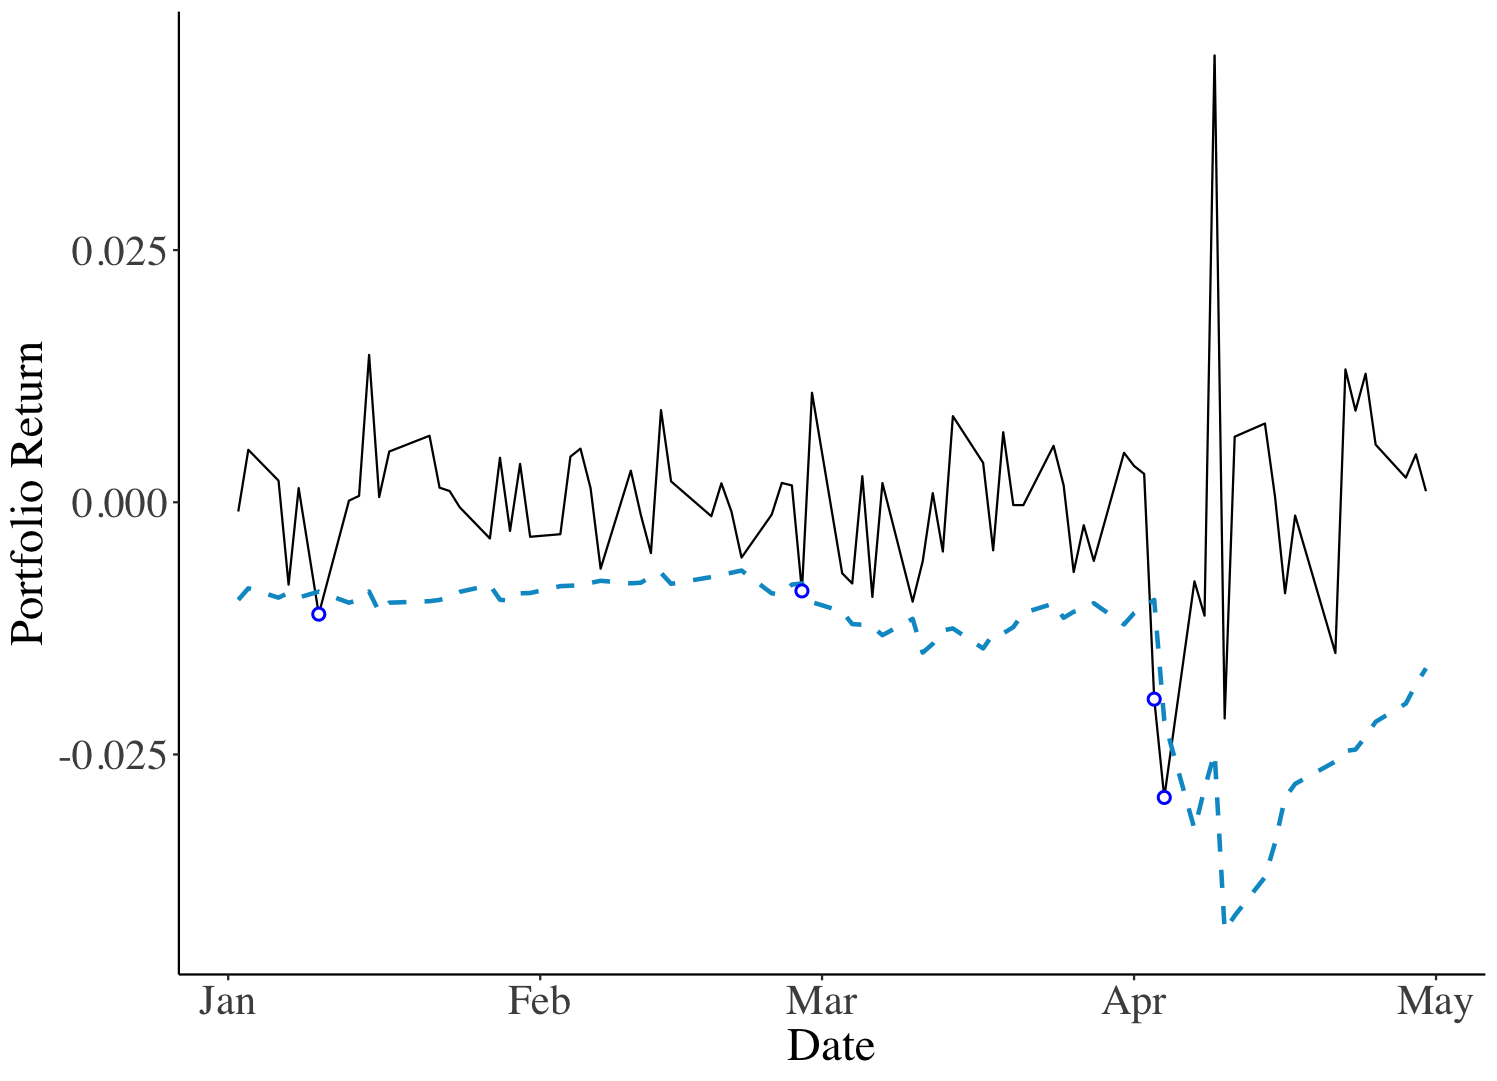
\includegraphics[scale=0.18]{../../plots/5.6.png} % Replace 
   \caption{2.5\% VaR breaches, GARCH-GACRH Copula.}
    \label{5.6}
\end{figure}

\begin{figure}[H]
    \centering
    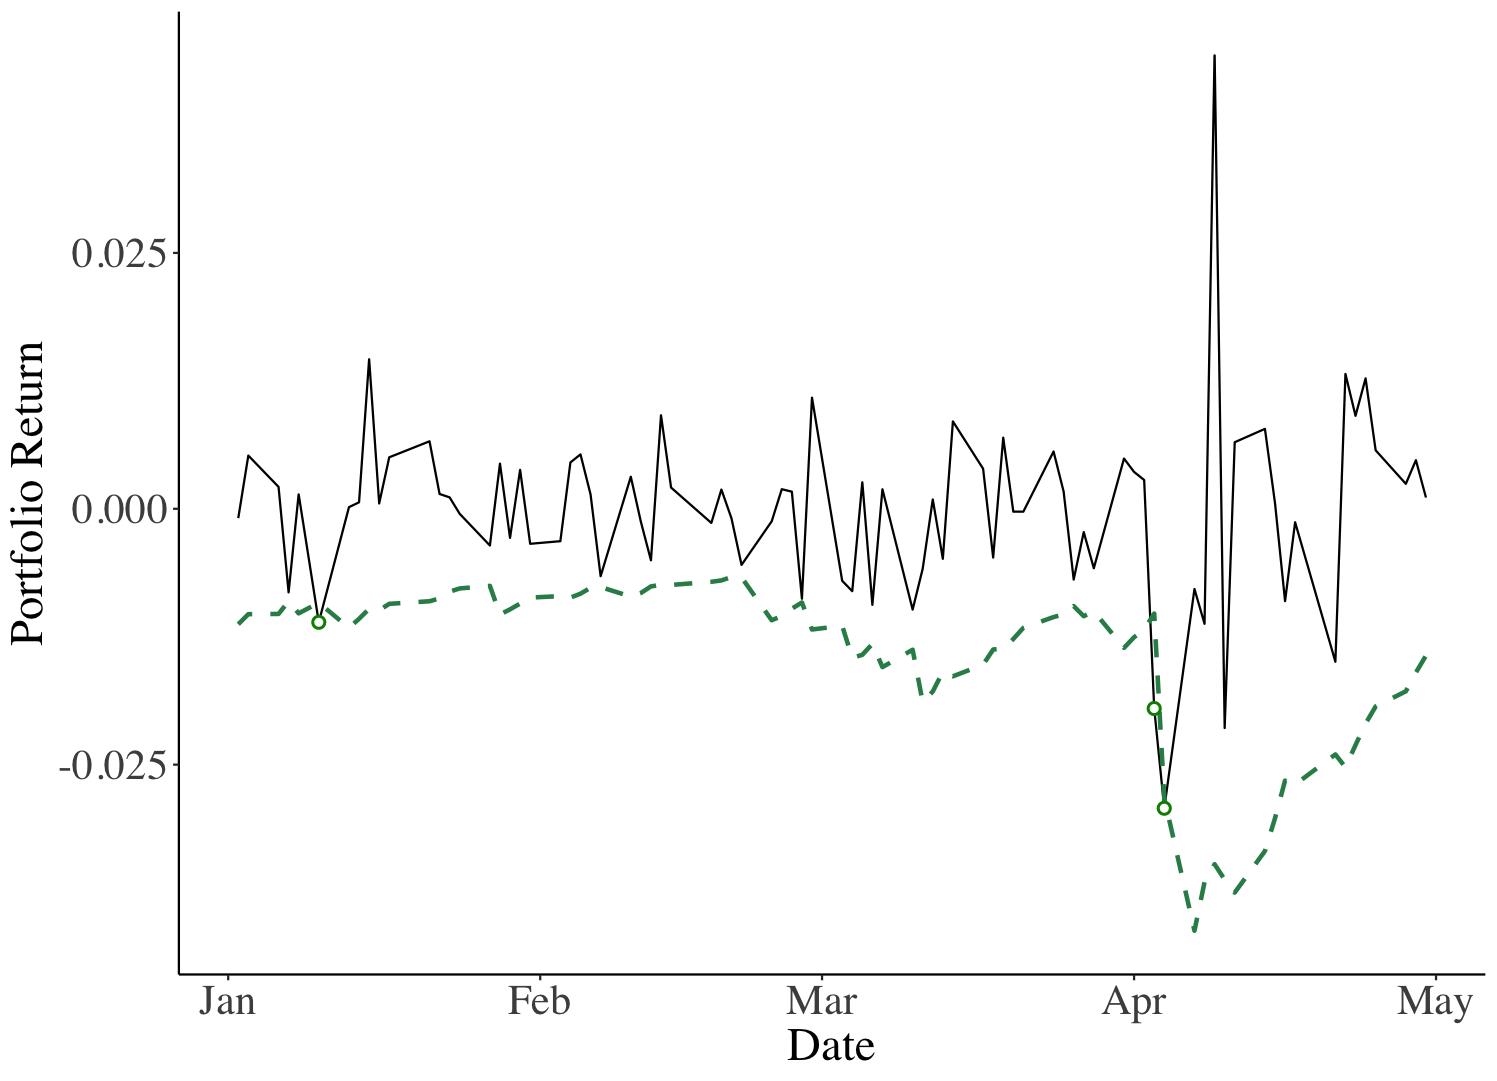
\includegraphics[scale=0.18]{../../plots/5.7.png} % Replace 
   \caption{2.5\% VaR breaches, GJR-GJR Copula.}
    \label{5.7}
\end{figure}

\begin{table}[htbp]
\centering
\begin{tabular}{llcc}
\toprule
\textbf{Test} & \textbf{p-value} & \textbf{GARCH-GARCH} & \textbf{GJR-GJR} \\
\midrule
$LR_{\text{uc}}$   & Theoretical & 0.2138 &  0.5168 \\
                   & Simulated   & 0.188 &  0.554 \\
$LR_{\text{ind}}$  & Theoretical & 0.1582 & 0.0729 \\
                   & Simulated   & 0.03 & 0.013 \\
$LR_{\text{cc}}$   & Theoretical & 0.1706 & 0.1622 \\
                   & Simulated   &  0.217 & 0.2 \\
\bottomrule
\end{tabular}
\caption{Theoretical and simulated $p$-values for VaR testing statistics.}
\label{tab:5.3}
\end{table}

Next, the statistical validity of the copula models is evaluated by examining the portfolio PIT histograms presented in Figures \ref{5.8} and \ref{5.9}. No significant deviations from uniformity are apparent. Performing a Kolmogorov–Smirnov test on the normally transformed PIT values, following the procedure described in \hyperref[chap:4]{Chapter4}, yields $p$-values of 0.5271 for the GARCH-GARCH model and 0.4872 for the GJR-GJR model. These results suggest that the Monte Carlo-generated densities constitute valid density forecasts for the portfolio returns. Figures \ref{5.10} and \ref{5.11} further illustrate the validity by comparing the empirical CDFs of the normally transformed PIT values against the theoretical standard normal CDF, highlighting the K-S test statistic.

\begin{figure}[H]
    \centering
    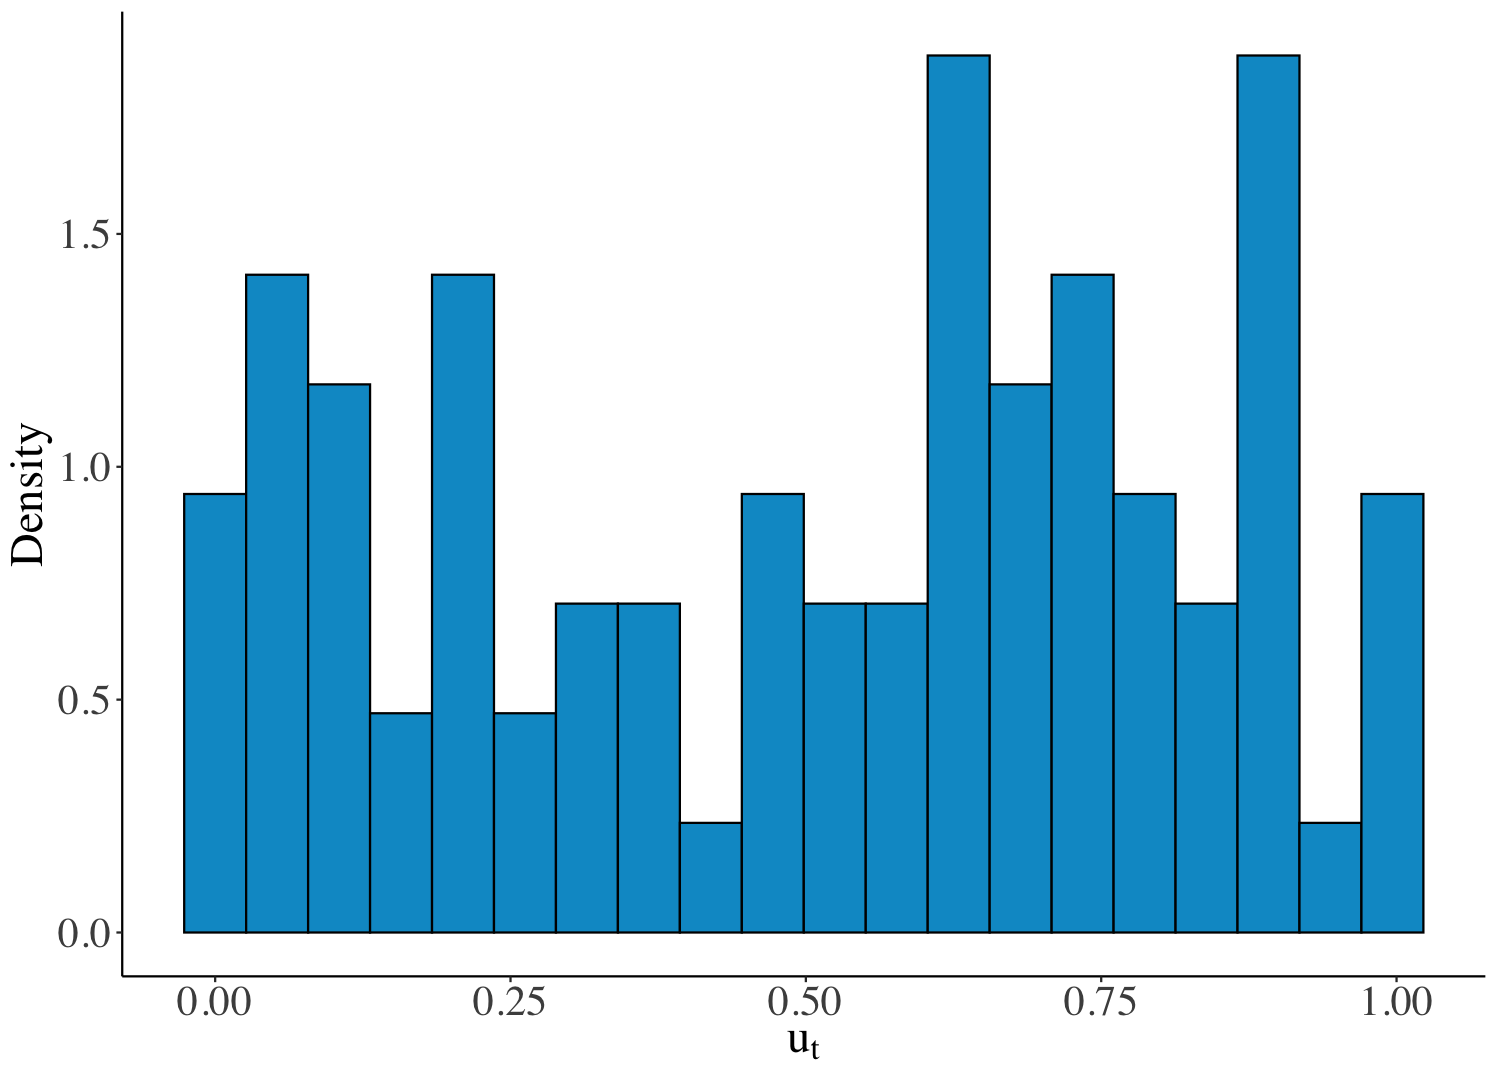
\includegraphics[scale=0.18]{../../plots/5.8.png} % Replace 
   \caption{Histogram of PIT values, GARCH-GARCH copula.}
    \label{5.8}
\end{figure}

\begin{figure}[H]
    \centering
    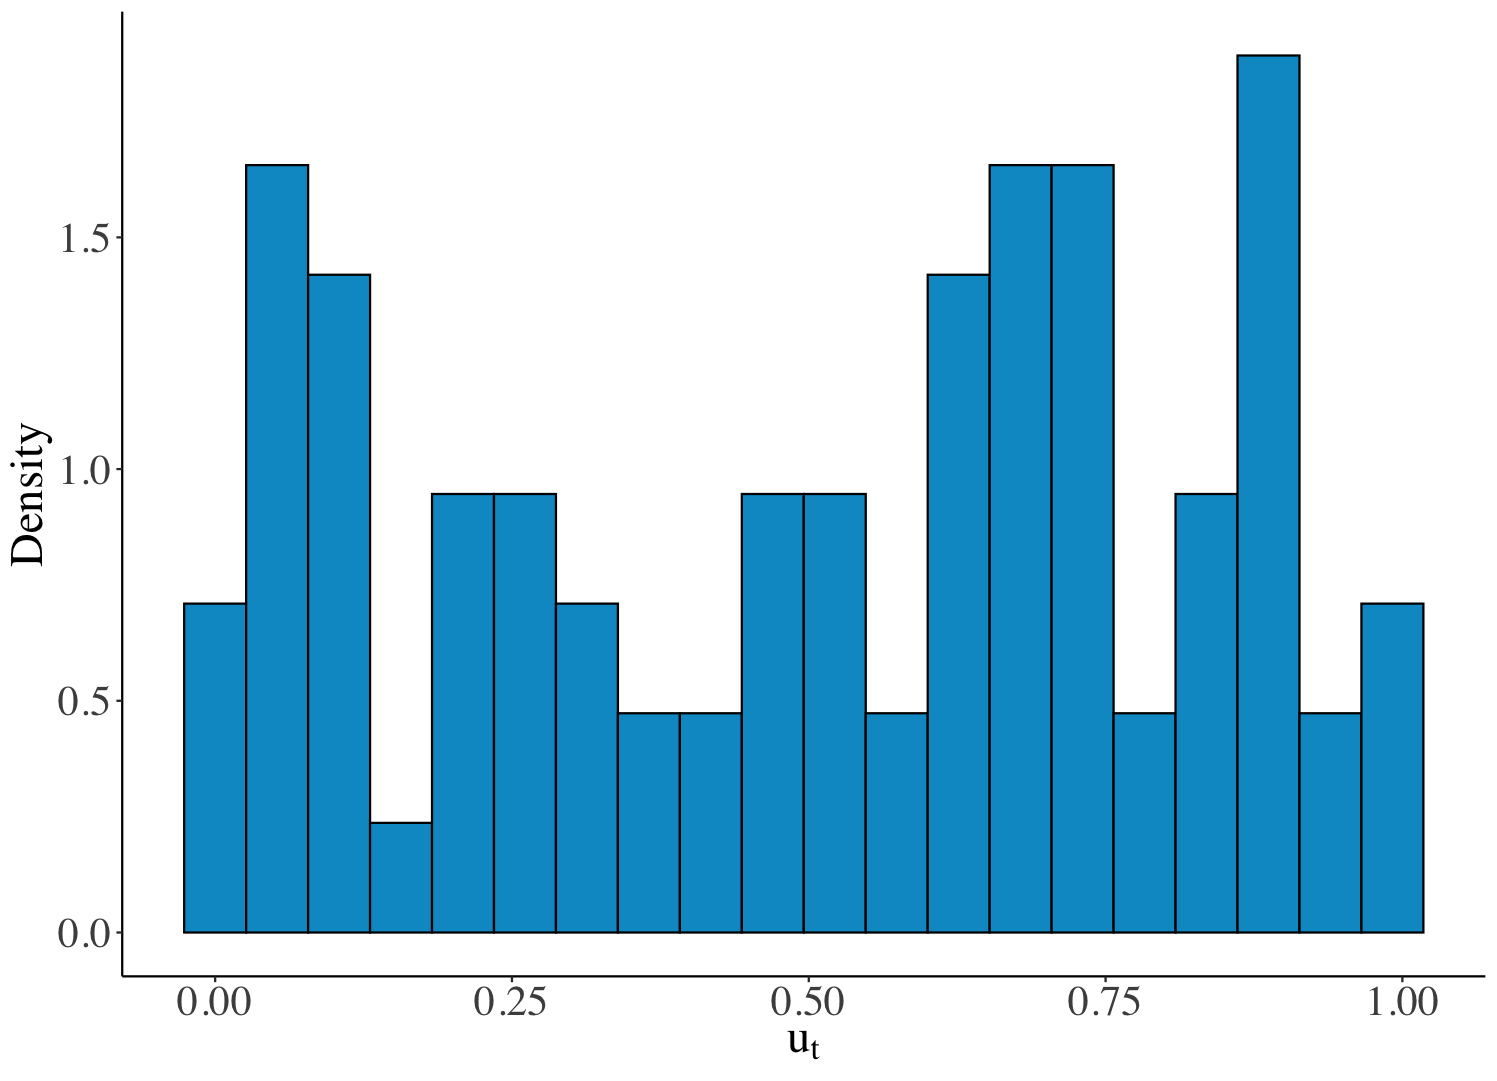
\includegraphics[scale=0.18]{../../plots/5.9.png} % Replace 
   \caption{Histogram of PIT values, GJR-GJR copula.}
    \label{5.9}
\end{figure}

\begin{figure}[H]
    \centering
    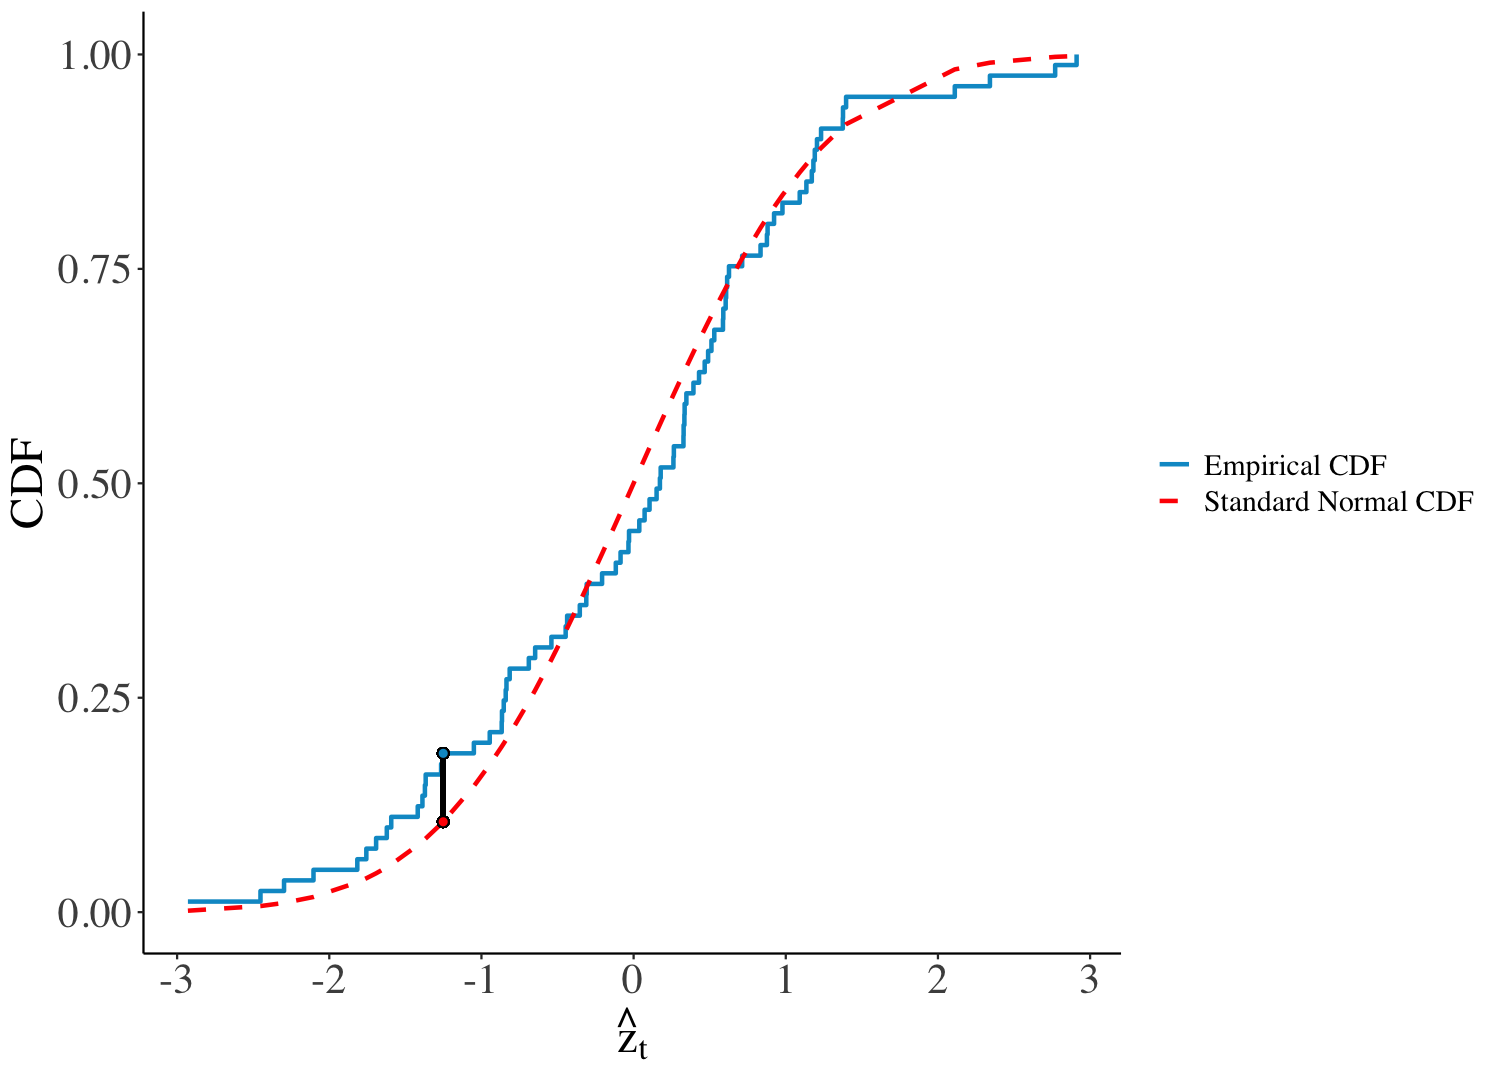
\includegraphics[scale=0.18]{../../plots/5.10.png} % Replace 
   \caption{Kolmogorov-Smirnov test on $\hat{z}_{t+1}$, GARCH-GARCH copula}
    \label{5.10}
\end{figure}

\begin{figure}[H]
    \centering
    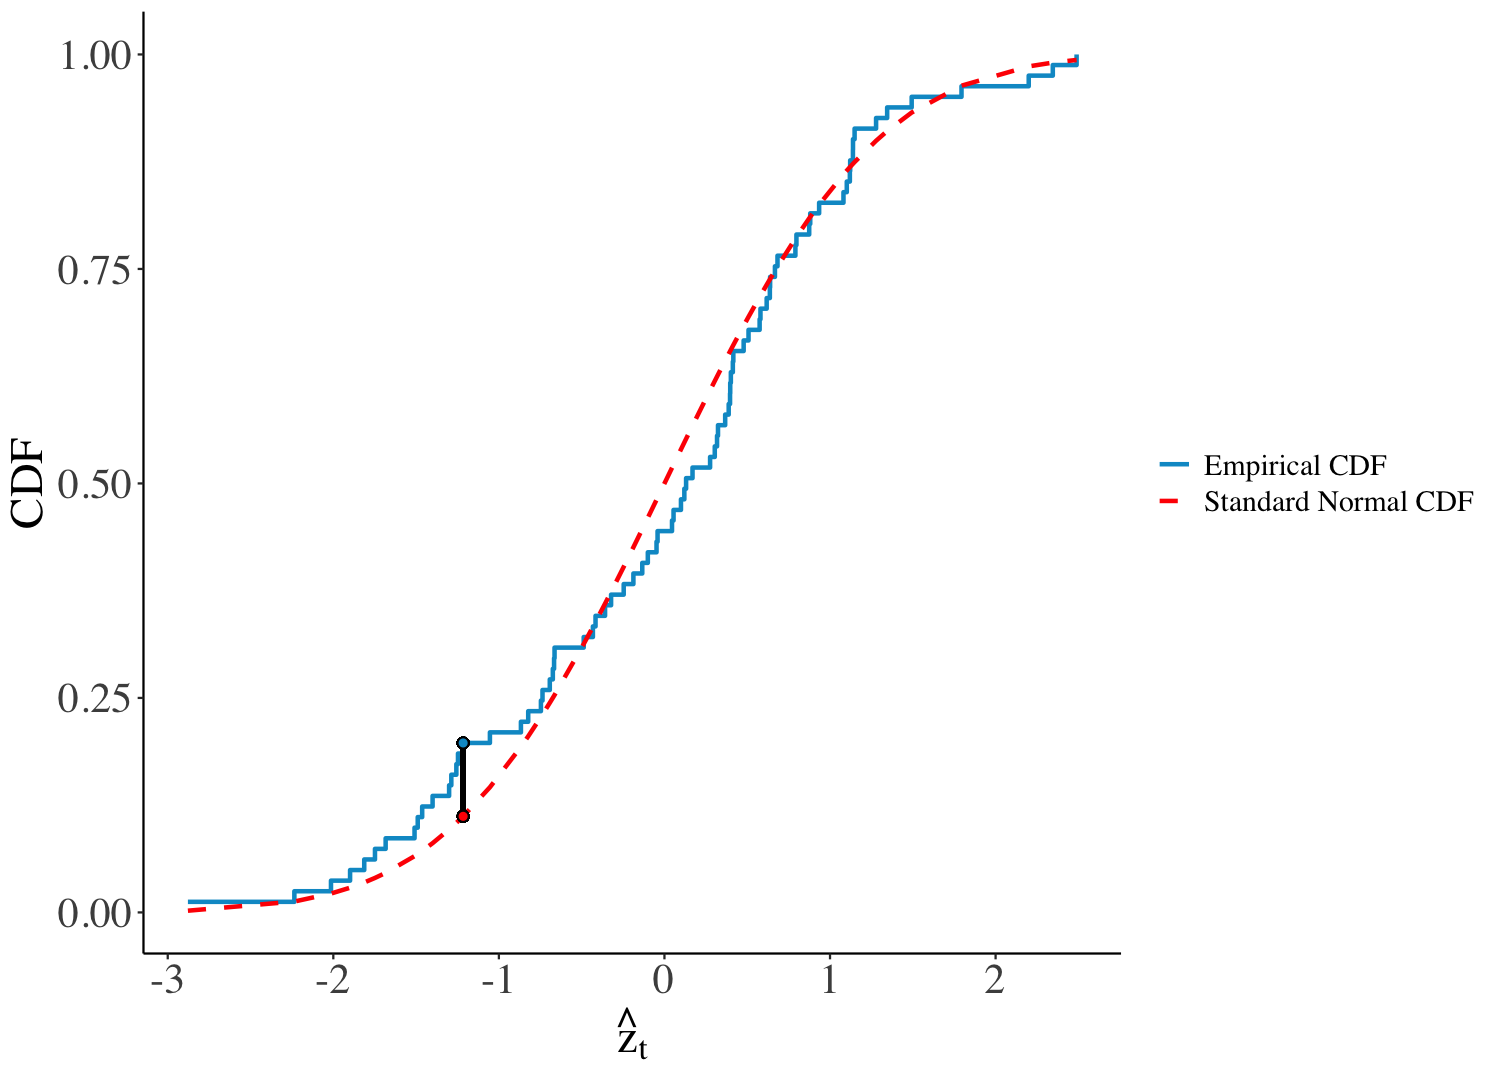
\includegraphics[scale=0.18]{../../plots/5.11.png} % Replace 
   \caption{Kolmogorov-Smirnov test on $\hat{z}_{t+1}$, GJR-GJR copula}
    \label{5.11}
\end{figure}

To conclude, copula models offer two main advantages. First, they allow univariate models for individual asset returns to be estimated independently, leveraging a wide and accessible body of literature. This flexibility makes complex univariate modeling more manageable. Second, copula models effectively capture nonlinear dependencies between asset returns, which are especially important from a risk management perspective. At the same time, the approach considered in this chapter has important limitations. The static symmetric $t$-copula is unable to capture the time variation in cross-asset dependence documented earlier, and its symmetry prevents it from fully reproducing the asymmetric tail dependence suggested by the threshold correlation plots. Moreover, the resulting VaR forecasts still adapt too slowly to abrupt changes in volatility. Thus, while the copula framework represents a practical and powerful approach to multivariate modeling, more flexible dynamic and asymmetric copula specifications appear necessary for a fuller description of the dependence between financial assets.

\newpage